%!TEX root = ../index.tex
Anwendungen welche mit externen Systemen kommunizieren, müssen auf einem Standard aufbauen welcher auch zukünftig noch unterstützt wird. Darum wurden zuerst die verschiedenen Standards betrachtet und danach mittels einer Nutzwert-Analyse ein System ausgewählt. Ein wichtiger Punkt für die Wahl eines Standards ist, dass die Integration in ein bestehendes Projekt möglichst einfach mit wenig Konfigurationsaufwand erreicht werden kann.

\section{Wahl eines Systems}
\label{sec:Wahl eines Systems}
Es gibt diverse Standards mit welchen man einen Benutzer identifizieren kann. Jedoch sind nicht alle davon für Webapplikationen geeignet. Um die Übersicht zu wahren, wird hier nur auf zwei Typische Web Standards eingegangen. Damit auch eine Authentifizierung über Mac OS X Server erreicht werden könnte, wird zusätzlich noch kurz auf LDAP eingegangen.

\subsubsection{OpenID}
\label{ssub:OpenID}
Der offene Standard Openid wird von der OpenID
Foundation\footnote{\url{http://openid.net/foundation/}}, welche dafür gegründet wurde Marketing zu betreiben und die Rechte an der Marke OpenID zu wahren, gepflegt. Der Standard wurde dafür entwickelt, es einem Benutzer welcher über eine OpenID verfügt zu ermöglichen sich an Webseiten welche OpenID unterstützen anzumelden, ohne dass er sich einen neuen Benutzername und ein neues Passwort ausdenken muss. Das System welches die OpenID zur Verfügung stellt, wird dabei \gls{OpenID-Provider} und die Webseiten an der sich der Benutzer anmeldet \glspl{OpenID-Relying-Party} genannt.

OpenID ist weit verbreitet und wird von vielen grösseren Webportalen unterstützt. Normalerweise erhält die \gls{OpenID-Relying-Party} nach dem ein Benutzer über OpenID eingeloggt hat, einen Identifier in form einer URL. Mit der attribute exchange Erweiterung lassen sich weitere Informationen über den Benutzer vom \gls{OpenID-Provider} beziehen.

\subsubsection{OAuth}
\label{ssub:OAuth}
Auch OAuth\footnote{\url{http://oauth.net}} ist ein offener Standard und ist zur Zeit in der Version 1.0 im RFC 5849\cite{rfc5849} aktuell. Jedoch verwenden die meisten Dienste heute schon OAuth 2.0 welches als Working Draft\footnote{\url{http://tools.ietf.org/html/draft-ietf-oauth-v2-26}} verfügbar ist. OAuth ist nicht für Authentifizierung gebaut sondern für Autorisierung. Es ermöglicht einem Benutzers einer Webapplikation die Vergabe von Rechten an einen weiteren Dienst, damit dieser bei der ersten Webapplikation API Funktionen aufrufen kann, auf welche er ohne das Einverständnis des Benutzers keinen Zugriff hätte. Es lässt sich mit OAuth eine Pseudo-Authentifizierung durchführen, welche darauf beruht, dass nur der Benutzer diese Rechte erteilen kann. Dieses System wird von Facebook für die ``Login with Facebook'' verwendet.

\subsubsection{LDAP}
\label{ssub:LDAP}
Obwohl es unüblich ist für Webapplikationen LDAP\cite{rfc4511} zu verwenden, wurde diese Variante ebenfalls geprüft, da dies der einzige praktikable Weg wäre um eine Single-Sign-On Lösung mit einem Mac OS X Server als Kontenverwaltungsdienst zu erstellen.

\section{Nutzwert-Analyse}
\label{sec:Nutzwert-Analyse}
Da mehrere Systeme in der allink vorhanden sind, welche sich für ein zentrales Login eignen, wurde eine Nutzwert-Analyse durchgeführt um die einzelnen Systeme miteinander zu vergleichen. Dabei wurde vor allem Wert darauf gelegt, dass sich die Mitarbeiter nicht ein weiteres Login merken müssen.

\subsection{Gewichtung}
\label{sub:Gewichtung}
Die Gewichtung der einzelnen Punkte wurde in Zusammenarbeit mit der allink Geschäftsleitung erarbeitet. Jedoch war zu diesem Zeitpunkt noch nicht bekannt, welches System bei welchem Punkt seine Stärken ausspielen kann. Die so festgelegte Gewichtung ist in Abbildung~\ref{fig:nutzwertanalyse gewichtung} zu sehen.

\begin{figure}[H]
    \centering 
		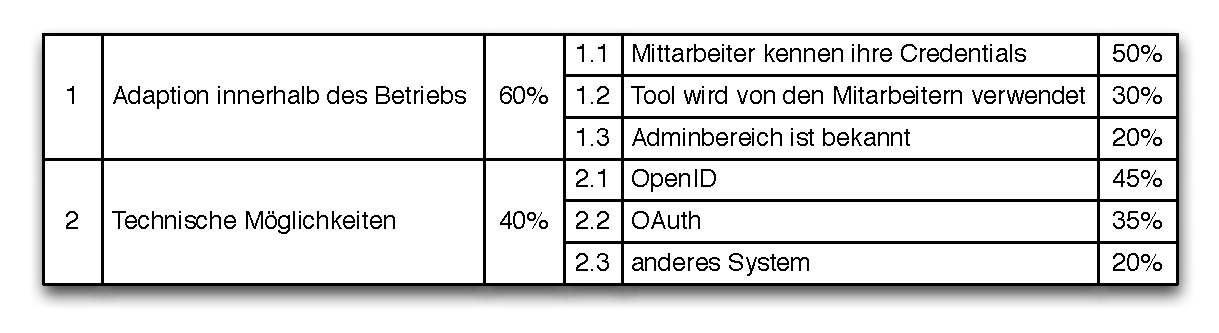
\includegraphics[width=1\textwidth]{include/nutzwertanalyse1.pdf}
		\caption{Gewichtung der einzelnen Faktoren}
		\label{fig:nutzwertanalyse gewichtung}
\end{figure}

\subsection{Bewertung}
\label{sub:Bewertung}
Die zuvor beschriebenen Systeme, wurden gemäss der in der Gewichtung genannten Punkte bewertet. Jeder Punkt der Nutzwert-Analyse wurde nach der Skala in Tabelle~\ref{tab:nutzwertanalyse skala} klassiert. Nachfolgend wird auf die einzelnen Punkte eingegangen.

\begin{table}[h]
    \centering
        \begin{tabular}{|c|l|}
        \hline
        0 & Punkt nicht erfüllt\\
        \hline
        1 & Punkt ungenügend erfüllt\\
        \hline
        2 & Punkt genügend erfüllt\\
        \hline
        3 & Punkt erfüllt\\
        \hline
        4 & Punkt mehr als erfüllt\\
        \hline
        \end{tabular}
		\caption{Skala für die Punktevergabe}
		\label{tab:nutzwertanalyse skala}
\end{table}


\subsubsection{Mitarbeiter kennen ihre Credentials}
\label{ssub:Mitarbeiter kennen ihre Credentials}
Das System soll den Mitarbeitern die Arbeit erleichtern. Die Bewertung für diesen Punkt wurde anhand der Umfrage aus Kapitel~\ref{sec:Mitarbeiter} erstellt.

\begin{tabular}{lc}
Google Apps & 3\\
Basecamp & 2\\
Mac OS X Server & 1\\
\end{tabular}

\subsubsection{Tool wird von den Mitarbeitern verwendet}
\label{ssub:Tool wird von den Mitarbeitern verwendet}
Unter diesem Punkt wurde beurteilt von wie vielen Mitarbeitern das geprüfte System bereits im Arbeitsalltag eingesetzt wird.
\paragraph{Google Apps}
\label{par:1.2Google Apps}
wird zur Zeit von allen Mitarbeitern verwendet, da darüber die E-Mail Dienste laufen. Zudem verwendet die IT und die Geschäftsleitung Google Docs und Google Sites.
\paragraph{Basecamp}
\label{par:1.2Basecamp}
wird vor allem von der Projektleitung verwendet. Der Rest der Mitarbeiter verwendet Basecamp vor allem für die Zeiterfassung, welche aber über ein Widget geschieht und so nicht viel mit Basecamp zu tun hat.
\paragraph{Mac OS X Server}
\label{par:1.2Mac OS X Server}
wird von allen Mitarbeitern für den Austausch von Dateien und für das Backup verwendet. Jedoch sind sich die meisten Mitarbeiter nicht bewusst wo sie dieses System verwenden, da sie sich dafür nie anmelden müssen.

\begin{tabular}{lc}
Google Apps & 4\\
Basecamp & 2\\
Mac OS X Server & 2\\
\end{tabular}

\subsubsection{Administrations-Bereich ist bekannt}
\label{ssub:Adminbereich ist bekannt}
Bei jedem Zu- und Abgang eines Mitarbeiters bei allink muss ein Benutzerkonto errichtet bzw. ein Benutzerkonto wieder gesperrt werden. Darum ist es notwendig, dass zumindest die Geschäftsleitung mit den entsprechenden Tools vertraut ist.
\paragraph{Google Apps}
\label{par:1.3Google Apps}
wird von der Informatik Leitung regelmässig verwendet. Daneben wird regelmässig Google Apps für Kunden eingerichtet und jeder Informatiker kennt sich im Administrationsbereich aus. Zudem sollte auch die gesamte Geschäftsleitung über Grundkenntnisse verfügen.
\paragraph{Basecamp}
\label{par:1.3Basecamp}
wird vor allem von der Projektleitung verwaltet. Das Erstellen eines neuen Mitarbeiters ist jeweils die Aufgabe der Informatik Leitung.
\paragraph{Mac OS X Server}
\label{par:1.3Mac OS X Server}
wird nur von der Informatik Leitung konfiguriert und wird sonnst von niemandem verwendet.

\begin{tabular}{lc}
Google Apps & 4\\
Basecamp & 2\\
Mac OS X Server & 1\\
\end{tabular}

\subsubsection{OpenID}
\label{ssub:Bewertung OpenID}
OpenID ist die erste Wahl, da es in Python schon unterstützt wird und es dafür konzipiert ist Benutzer über ein zentrales System anzumelden.
\paragraph{Google Apps}
\label{par:2.1Google Apps}
unterstützt OpenID und wird auch auf der Webseite der OpenID Foundation gelistet.
\paragraph{Basecamp}
\label{par:2.1Basecamp}
unterstützte früher OpenID hat jedoch die Unterstützung am 1. Mai 2011 \footnote{\url{http://productblogarchive.37signals.com/products/2011/01/well-be-retiring-our-support-of-openid-on-may-1.html}} eingestellt.
\paragraph{Mac OS X Server}
\label{par:2.1Mac OS X Server}
unterstützt ohne zusätzliche Software kein OpenID.

\begin{tabular}{lc}
Google Apps & 3\\
Basecamp & 0\\
Mac OS X Server & 1\\
\end{tabular}

\subsubsection{OAuth}
\label{ssub:Bewertung OAuth}
Obwohl OAuth eigentlich nicht als authentifizierungs Protokoll gedacht ist. Kann es dafür verwendet werden indem man vom Provider die entsprechenden Daten bezieht. Dies ist jedoch zweite Wahl falls sich keine Möglichkeit bietet OpenID zu verwenden.
\paragraph{Google Apps}
\label{par:2.2Google Apps}
lässt über OAuth Zugriff auf Benutzerdaten und Schnittstellen zu.
\paragraph{Basecamp}
\label{par:2.2Basecamp}
lässt über OAuth Zugriff auf die gesamte API zu.
\paragraph{Mac OS X Server}
\label{par:2.2Mac OS X Server}
unterstützt kein OAuth.

\begin{tabular}{lc}
Google Apps & 3\\
Basecamp & 3\\
Mac OS X Server & 0\\
\end{tabular}

\subsubsection{anderes System}
\label{ssub:anderes System}
Für den Fall, dass keines unserer Systeme geeignet ist um einen Benutzer mit OpenID oder OAuth zu authentifizieren, wurden weitere Möglichkeiten unserer Systeme überprüft.
\paragraph{Google Apps}
\label{par:2.3Google Apps}
bietet neben den schon erwähnten Möglichkeiten noch Unterstützung für SAML\footnote{\url{http://www.oasis-open.org/committees/tc_home.php?wg_abbrev=security}} jedoch zur Zeit nur um Benutzer von Google Diensten über ein Drittsystem zu authentifizieren.
\paragraph{Basecamp}
\label{par:2.3Basecamp}
bietet keine weitere Möglichkeiten an.
\paragraph{Mac OS X Server}
\label{par:2.3Mac OS X Server}
hat standardmässig einen LDAP Dienst integriert. Darüber könnte man die nötige Authentifizierung und Autorisierung tätigen.

\begin{tabular}{lc}
Google Apps & 1\\
Basecamp & 0\\
Mac OS X Server & 3\\
\end{tabular}

\section{Auswertung}
\label{sec:Auswertung}
Wenn man die obigen Bewertungen gewichtet und summiert zeit sich ein klarer Sieger. Dies lässt sich dadurch erklären, dass Google die eigene Platform bewusst mit den nötigen Schnittstellen ausrüstet, weil es für Google Apps mittlerweile sogar einen Marktplatz für Zusatztools gibt.

\begin{table}[h!]
  \centering
  \begin{tabular}{|l|lr|lr|lr|lr|lr|lr|r|}
  \hline
  System & 1.1 & 0.3 & 1.2 & 0.18 & 1.3 & 0.12 & 2.1 & 0.18 & 2.2 & 0.14 & 2.3 & 0.08 & Total\\
  \hline
  Google Apps & 3 & 0.9 & 4 & 0.72 & 4 & 0.48 & 3 & 0.54 & 3 & 0.42 & 1 & 0.08 & 3.14\\
  \hline
  Basecamp & 2 & 0.6 & 2 & 0.36 & 2 & 0.24 & 0 & 0 & 3 & 0.42 & 0 & 0 & 1.62\\
  \hline
  Mac OS X Server & 1 & 0.3 & 2 & 0.36 & 1 & 0.12 & 1 & 0.18 & 0 & 0 & 3 & 0.24 & 1.2\\
  \hline
  \end{tabular}
  \caption{Auswertung der Nutzwertanalyse}
  \label{tab:auswertung_nutzwertanalyse}
\end{table}